\documentclass{acm_proc_article-sp}
\usepackage{amsfonts}
\usepackage[ruled,vlined]{algorithm2e}
\usepackage{epsfig}
\usepackage{mathrsfs}
\usepackage{multirow}
\usepackage{slashbox}
\usepackage{booktabs}
%\usepackage{subfigure}
% some very useful LaTeX packages include:
\usepackage{CJK}
%\usepackage{cite}      % Written by Donald Arseneau
%\usepackage{graphicx}  % Written by David Carlisle and Sebastian Rahtz
\usepackage{color}
\usepackage{psfrag}    % Written by Craig Barratt, Michael C. Grant,
\usepackage{subfigure} % Written by Steven Douglas Cochran
\usepackage{url}       % Written by Donald Arseneau
\usepackage{stfloats}  % Written by Sigitas Tolusis
\usepackage{amsmath}   % From the American Mathematical Society
\usepackage{array}
\usepackage{amssymb}
%\usepackage{algorithm}
\usepackage{{inputenc}}
\usepackage{balance}
\usepackage{amsmath}
\usepackage{multirow,tabularx}
\usepackage{balance}
%\usepackage[dvips]{graphicx}
\usepackage{longtable}
\usepackage{booktabs,longtable}
\newcommand{\vectornorm}[1]{\left|\left|#1\right|\right|}
\newcommand{\tabincell}[2]{\begin{tabular}{@{}#1@{}}#2\end{tabular}}
\newcommand{\bpi}{\boldsymbol{\pi}}
\usepackage[ruled]{algorithm2e}
\usepackage{color}
\usepackage{dsfont}
\hyphenpenalty=5000
\tolerance=5000


\begin{document}

%\title{\#Diabetes on Twitter: A Characterization Study through Big Data}
\title{\#Bgnow on @Twitter: A Characterization Study of \#Diabetes through \#BigData}
%\subtitle{Paper ID: 240}
%Diabeteson Twitter: A Success Characterization Study through Big Data
\maketitle
\begin{abstract}
Social media is continually used as a platform for sharing, seeking, and discussing around health challenges, transforming these platforms as a source for knowledge, support, and engagement for patient living with chronic diseases. Studying behavioural characteristic and the language of users online can offer invaluable insights on how health consumers interacts and influence each other on social networks. In this paper, we investigate to characterize the differences between language and behaviour of diabetic users on Twitter microblogging platform. In particular, we aim to investigate the behavioural distinction between patients who can successfully manage their diabetes and those who fail. We study patient behavioural online in terms of linguistic, textual and visual attributes and contents in their online posts. We have observed several characteristics such as negative affective, seeking and sharing supportive contents, and difference in shared visual concepts, which differs adopted and non-adopted users. We discuss the implication of our finding in providing better healthcare intervention and provide a supervised model which can predict the success of user based on his published online content.

\end{abstract}

% A category with the (minimum) three required fields
\category{H.3.3}{Information Storage and Retrieval}{Information Search and Retrieval-clustering}
%A category including the fourth, optional field follows...
%\category{D.2.8}{Software Engineering}{Metrics}[complexity measures, performance measures]

\terms{Algorithms, Performance, Experimentation}


\keywords{Health informatics} % NOT required for Proceedings

\section{Introduction}

%Background: increase use of social media, qualtified self and health in social media, invaluable platform for studying indivicuals and communities' wellness
Social media has been considered as a prominent means for seeking, sharing and spreading information, where users discuss about a verity of events and topic of their interests. In such a context, health consumers increasingly utilize social platforms to fulfill their health demands through seeking and sharing health information and experiences as well as providing online social support for their peers~\cite{attai2015twitter,de2014seeking,dredze2012social}. For example, it was reported that $57\%$ of patients with chronic conditions constantly and actively refer to social media to acquire health information while $20\%$ of them have already participate in generation of online health contents~\cite{socialmediaandhealth}. In essence, social environments and virtual communities have been transformed to a confident environment permitting users to be connected with their peers who have experienced similar conditions, difficulties, and challenges, assisting them to cope with their situations~\cite{davis2015seeking,greene2011online}. The emerging of self-tracking gadgets and the enthusiasm of users in taking informed health decisions have also intensified this trend. This motivates users to not only share about their daily life events but also disclose their health information in social platforms \cite{de2013predicting}. For example diabetic patients frequently posts about their health conditions, medications, and the outcome of medications on social media platforms like Twitter and Instagram. Further, the ubiquity of social media encourages  health consumers to not only discuss about their health conditions and share experiences but more importantly share their health related measurements, like blood pressure and blood glucose, which provides an invaluable resource to study and analysis individual's and communities' wellness and behaviour. While Electronic Health Records (EHRs) are increasingly utilized in medical informatics as an important and distinct data source, limited research efforts have been devoted into utilizing PGWD available on social networks~\cite{che2015distilling,robinson2012deep,sun2015linkage}.

%Talking about Diabetes rise, the importance of self-management, factors involves in success of individuals in diabetes management,
Diabetes is the sixth leading cause of death in the US and it is estimated to be the seventh cause of the worldwide by $2030$~\footnote{\url{http://www.cdc.gov/diabetes/data/statistics/2014statisticsreport.html}}. It causes serious complications and can lead to poor quality of life \cite{american2012standards}. People with diabetes are more suspectable to other illnesses. However, they can reduce the occurrence of these potential complications through diabetes self-management. Training and education of self-management of diabetes prevent unnecessary health care utilization and hospitalization and improve patients wellness~\cite{haas2013national}. However, diabetes self-management is not a trivial task for chronic patients since it is highly linked to several individual and cultural factors such as demographic attributes, psychological mood, patient knowledge and lifestyle. The prominent role of self-management in diabetes has resulted into the emergence of several diabetes management programs and schemes~\cite{haas2013national}. However, the success and efficacy of this programs are still unclear or partially opaque due to the following reasons~\cite{garrett2005patient,lorig2010online}. First, most of these studies have been performed in a controlled clinical setting and only investigate some of health factors of interest like diet and activities. Even though these factors are important the effects can vary from patient to patient making the reported results almost restricted to the local community studied. Second, the adherence of the user is a major factor in these program. However, users adherence and ambitious vary from time to time making the generalization of result optimistic.
%There is evidences of that users tend to more adhere to the self-management program when they are under inspection.
Third, traditional studies in health sciences are mostly based on a observational study or based on survey data from patients which are limited in the number of subjects and the time period of the study, making it hard to derive a comprehensive conclusion. Therefore, the factors affect on success of users in managing their diabetes are still not fully studied. In particular, the role of personal characteristics like user's behavior and mood is still unclear.

%research aim + research question
In this paper, we investigate the success of users to self-manage their diabetes, the role of users' behavior on self-management, and how exactly this behavior correlates to self-management and health of user.% In particular, we study the factors which differentiate the online behaviour of diabetes patients who can self-manage their diabetes in terms of blood glucose value.
In particular, we investigate the factors which differentiate two cohorts of users: Adopted and Non-Adopted diabetes patients, where they are divided by their success in controlling their blood glucose values on healthy target range.
In contrast to traditional studies, we utilize users self-mention values of blood glucose on Twitter microbloging service. We study users from three aspects, namely linguistic attributes, published textual content, and shared multimedia contents, i.e., images on Instagram, to find their behavioural distiction.  Specifically, we address the following research questions:
\begin{itemize}
\item [\textbf{RQ1:}] What are the characteristics of these communities in terms of linguistic, behavioural, cognitive and affective styles and attributes?
\item [\textbf{RQ2:}] How do they differ in terms of their posts content published in social platforms?
\item [\textbf{RQ3:}] How different are their multimedia interests on social platforms, i.e. what entities and concepts do they often share in pictures on social networks?
\end{itemize}

% importance of this research
Studying behavioural characteristics of successful patients provides significant insight about individual's wellness. First, understanding behaviour factors correlated with success in managing diabetes will help us to design proper intervention program to assist users coping with their condition and improve their wellness. Second, by understanding success factors in self-management, we can assist new diagnosed users as well as users struggling with their condition to adopt their lifestyle with the disease condition. Third, several years of research in user behaviour and wellness have clearly revealed that social networks and health are closely related through the social reinforcements come from observing and modeling others' behaviors \cite{ruths2014social}. By linking users in different categories, i.e. suggesting successful users to strugglers, we can assist them to learn positive behaviours from new friend on social communities~\cite{maibach1995moving,korda2013harnessing,hawn2009take}. This study is also beneficial for understanding collaborative behaviour of communities. By aggregating behaviour of individuals, we can shed light on public health, trying to understand the wellness patterns and trends of user groups in large scale. Overall, the answers to these questions will enhance our understanding of users' online interactions about diabetes, in particular on the Twitter microblogging platform and Instagram multimedia sharing service, and how their behaviours are correlated with their health condition, assisting us in various applications like group wellness analysis~\cite{tang2011group}, public health~\cite{hawn2009take,luxton2012social}, and health policy~\cite{murray1996evidence}, to name a few.


%contribution of the research
The contribution of this paper are threefold:
\begin{itemize}
\item We demonstrate an effective approach for collecting patient generated wellness data from social media, which scale well. In particular, we introduce an approach for harvesting wellness information available on social media for studying diabetes and especially diabetes success.
\item We conducted a behavioural analysis of social media users who can successfully manage their diabetes and the factors which cause a fail.
\item We conduct an open vocabulary analysis that captures language use of diabetic patients toward identifying behavioural patterns result in self-managing diabetes.
\item We investigate media contents shared by diabetes patients to reveal their preferences in sharing various visual concepts.
\end{itemize}


Our results open a new research direction to study wellness in large scale utilizing social media data. Further, the study demonstrates the potential of social media to design proper intervention and treatment programs for diabetic patients. The remainder of this paper is organized as follows. In Section $2$, we review related studies which utilize social media for wellness. We next explain data collection approach and grand-truth construction in Section $3$. Section $4$ describes several analytical experiments we conducted in this paper followed by experimental results in Section $5$. In Section $6$, we conduct a success prediction study for diabetic patients followed by discussion in Section $7$. Finally, we summarize the paper and outline the future work in Section $8$.

% Extend this
%The aim of this paper is to analyze the semantic content of tweets discussing diabetes and diets, and the conversational connections of those tweeting and those being mentioned in the tweets

%Recently, online health communication that is dynamic, in contrast to static as traditional health-related resources are, offers users with certain conditions an opportunity to benefit from social networks to learn about the condition, and to be supported by others with similar experiences \cite{greene2011online}. Social networking tools offer the potential of supported learning, networking with peers, families and friends, as well as sharing problems, processes and outcomes with a global community \cite{some-paper}.
%
%Furthermore social networks and health are closely related through the social reinforcements come from observing and modeling others' behaviors \cite{ruths2014social}.
%
%This provides new opportunities for understanding and studying health in a scale which perviously was impossible.
%
%By mining the available Patient Generated Wellness Data (PGWD) on social media, we can gain invaluable insights into wellness of individuals as well as communities.
%While Electronic Health Records (EHRs) are increasingly utilized in medical informatics as an important and distinct data source, limited research efforts have been devoted into utilizing PGWD available on social networks\cite{ref-phenotypes}.
%%In such a context, social media platforms have been recently utilized to study various health conditions such as depression detection \cite{de2013predicting}, addiction recovery \cite{maclean2015forum77,murnane2014unraveling},  insomnia \cite{jamison2012can} and etc.
%
%
%
%%benefits of the research
%%challenges and problems






\section{Related Work}
% excessive use of social media for health and chronic diseases


\section{Data Collection and Ground-Truth Generation}
\subsection{Dataset}
We harvested public data available on social media for the construction of dataset as well as ground truth labels. We utilized a set of diabetic users who actively share their wellness information on Twitter and Instagram.  These users, besides posting about general topics and events, actively post their lifestyle information and activities such as their diet, activities, and emotional states. They further disclose their health information in terms of medical events and measurements like the onset of hypoglycaemia/heyperglocemia and their blood glucose values, respectively. A main characteristic of this cohort of users is that they report the exact values of their blood glucose in tweets using `\#BgNow' hashtag. This hashtag is popular among diabetic patients to report their blood glucose values and other diabetic related information online. In essence, `\#BgNow' plays the role of an online support group for diabetic patients through which they share, explore, and validate their health states and knowledge. The hashtag is special interest for us since it enables us to study  the correlation between diabetes patients behaviours  and their health indicators, e.g. blood glucose value. Indeed, \#bgnow hashtag acts as a social sensor through which we can measure the blood glucose values of individuals on social networks.

Analyzing this collection of tweets provides invaluable insight about diabetic patients and their health information disclose on social media  as well as the correlation between their behaviour online and their health conditions. We next collected all the published tweets in the period of six months from May to November $2015$ resulting into more than three million tweets. We next filter out all the users who did not post any status for one month or post few tweets. To link the twitter account of users with their Instagram, we obtained the cross-platform links in which they publish a post from their Instagram account on Twitter. By storing all these link, we can find their Instagram account and avoid the problem of user identification across different networks\cite{vosecky2009user}. It is worth noting that, by utilizing this approach, we may fail to find the corresponding Instagram for those users who are not post cross network, resulting into a smaller datast for Instagram. Table \ref{table::dataset-statistics} shows statistics of our datasets for both Twitter and Instagram.

Table \ref{table::sample-tweets} shows several representative tweets from the dataset. As you can see, there are three major tweet categories pertaining to diet, activity, and health information of individuals. It is worth noting that except these tweets, there are other tweets which may not directly related to health of individuals as demonstrated in the last row of Table \ref{table::sample-tweets}.


\subsection{Ground-truth Generation}


\begin{table}
\centering
%\vspace{-0.2em}
\caption{Statistics of the Dataset\label{table::dataset-statistics}}{
\footnotesize
\begin{tabular}{|c|c|c|}\hline
&\tabincell{c}{Twitter}&\tabincell{c}{Instagram}\\\hline
\tabincell{c}{\# of Users}&\tabincell{c}{$649$}&\tabincell{c}{$113$}\\\hline
\tabincell{c}{\# of Posts}&\tabincell{c}{$1,507,681$}&\tabincell{c}{$2,623$}\\\hline
\tabincell{c}{\# of Bgnow Posts}&\tabincell{c}{$20,079$}&\tabincell{c}{$-$}\\\hline
\tabincell{c}{Max Degree of the Users}&\tabincell{c}{$7,695$}&-\\\hline
\tabincell{c}{Min Degree of the Users}&\tabincell{c}{$1$}&-\\\hline
\tabincell{c}{Avg. Posts per Users}&\tabincell{c}{$2,323$}&\tabincell{c}{$17$}\\\hline
\end{tabular}}
%\vspace{-1.8em}
\end{table}


\begin{table}
\scriptsize
%\scriptsize
\centering
\caption{Examples of wellness tweets from dataset\label{table::sample-tweets}}{
\begin{tabular}{|c|}\hline
Diet \\ \hline
\tabincell{c}{Too much drink in party }\\
Talking about hot chocolates, I might just go and make myself one :D\\
found Taylor's pretzels in my backpack and I'm so happy wow\\
\tabincell{c}{Eat 20g carbs and go fo running}\\ \hline
Exercise \\ \hline
\tabincell{c}{after 1 hour run \#bgnow 130}\\
\tabincell{c}{I just finished 1 hour biking}\\
\tabincell{c}{BGnow 95, thanks swimming pool}\\ \hline
Health \\ \hline
\tabincell{c}{Feel too much Fatigue} \\
\tabincell{c}{ate great oatmeal, toast, and eggs. Had 1 unit insulin} \\ \hline
Others \\ \hline
\tabincell{c}{blood sugar taking a nosedive!  was it the symlin or the 10 mile run?} \\
\tabincell{c}{Can diabetics eat plums?: URL URL} \\
\tabincell{c}{A low sugar diet, I eat fruit? Some bad or better for me? URL} \\ \hline
\end{tabular}}
%  \vspace{-2.5em}
\end{table}

Medical studies suggests that diabetic users maintain their blood glucose between $70$ to $130$, which is considered as controlled blood glucose. A measurement between this range demonstrates that the patient could successfully manege his blood glucose while he was unsuccessful otherwise. The out of range values normally need to be corrected by lifestyle changes or treatments. Motivated by this principle, we partition the users into two distinct cohorts based on their reported blood glucose values: \textbf{Adapted Cohort} (\textbf{AC}), and \textbf{Non-adapted Cohort} (\textbf{NC}). The definition of these two cohorts are as follow,
\begin{itemize}
\item \textbf{Adopted Cohort (AC)}: An adapted user is able to control and maintain his values of blood glucose in the suggested range most of the times. For such a user, his blood glucose measurements are in the suggested range more than $t\%$ of times.
\item \textbf{Non-adopted Cohort (NC)}: A user is non-adopted if he fail to have a controlled blood glucose, i.e., his blood glucose measurements are usually out of range.
\end{itemize}

We set the threshold $t = 50$ to divide the users in our dataset into two groups of different blood glucose patterns. Mathematically, we utilized the following decision function to construct ground truth labels,
\begin{align}
\label{eg::decision-function-bg}
d(u_i) =
\begin{cases}
+1 \quad \text{if} \quad \frac{Pr(u_i \in AC)}{Pr(u_i \in NC)} \geq t\\
-1 \quad \text{otherwise}
\end{cases},
\end{align}
where $Pr(u_i \in AC)$, and $Pr(u_i \in NC)$ are the probability that the measurements for user $u_i$ are in the controlled range and out of the controlled range, respectively.
This grouping is coarse, but it is motivated by health studies~\cite{franciosi2001impact, malanda2013self} stating that users who can manage their blood glucose will have a better long term health and fewer diabetes complications. In the future, we aim to define more detailed groups, e.g., users who have on target, below target, above target measurements and also different trends like stable, and fluctuating trends.
By using Eq.(\ref{eg::decision-function-bg}), we can intuitively divide our diabetic patients into two groups of users, which clearly show how they have managed their diabetes. In the remainder of the paper, we study how these two communities' online behaviour differ in terms of linguistic, textual, and visual content published on their social network posts.

\subsection{Attribute Extraction}
The aim of our research is to investigate the behavioural distinction between two different cohorts of patients with respect to their health attributes, in our study blood glucose values. To do so, we need to extract the reported measurements of blood glucose values in their tweets. Several approaches have been proposed in information extraction to detect the right piece of information from a text corpus, like pattern-based methods, supervised classification, and Conditional Random Field (CRF) \cite{chang2006survey}. Here, we utilized a simple but effective rule based approach. Intuitively, we defined a set of regular expression to extract the measurement values of blood glucose for individuals as shown in Table \ref{table::regular-expression-examples}. We followed a bootstrapping approach of~\cite{thelen2002bootstrapping} to ensure the coverage and diversity of used patterns, where all extracted patterns are manually verified to ensure accuracy. Given a user post, we apply these set of rules to find whether a given tweet contains any reported valued of blood glucose\footnote{In some cases, several numerical values might be found as a candidate for blood glucose value. We used the value which is closer to \#Bgnow hashtag as the reference value.}.





\begin{table}
\scriptsize
\centering
\vspace{-0.2em}
\caption{Representative examples of regular expressions for extracting blood glucose values from users' posts.\label{table::regular-expression-examples}}{
\begin{tabular}{|m{3.15cm}|m{2.7cm}|m{1.4cm}|}\hline
\tabincell{c}{195.0 BG @ 08:20AM  \\ after bike ride 90 minutes} & NUMBER (mg|mmol) (BG|Bgnow)  (at|@) TIME * & \tabincell{c}{BG : 195\\Time: 08:20} \\\hline
\tabincell{c}{Going on a 3 mile run, \\\#BGnow 120 \#bigbluetest } & * (BG|BGnow) NUMBER &  \tabincell{c}{BG : 120} \\\hline
\end{tabular}}
\vspace{-0.2em}
\end{table}



\section{Content Analysis}
In this section, we applied different analytical experiments we applied for understanding the behavioural distinction between AC and NC users.
\subsection{LIWC Analysis}
To identify and understand behaviour distinction of adapted and non-adapted groups, we leverage a variety of indicators including linguistic and non-linguistic indicators.
The motivation behinds the investigation is that several psychological studies demonstrate behavioural expression of individuals and their responses expose their life context, crises, and vulnerabilities~\cite{pennebaker2001linguistic}. Our analysis, in this section, is largely based on LIWC, which has been widely used in literature to study individuals behaviours in depression \cite{de2013social}, addiction recovery \cite{maclean2015forum77}, anorexia \cite{de2015anorexia}, to name a few. We hence examine three categories of attributes named (1) affective attributes, (2) cognitive attributes and (3) linguistic and stylistic attributes.

\emph{Affective attributes}. Affective measures have attracted a lot of research in text and opinion mining to detect the objectivity of user towards products, organization, and services \cite{liu2012sentiment}. Recently, affective measures have been largely utilized to measure emotional disclosure of users in social media \cite{kumar2015detecting}. Motivated from prior literature, we measure positive affect (PA) and negative affect (NA) based on LIWC categories. We also compute four other emotional expression indicators: anger, anxiety, sadness, and swear.

\emph{Cognitive attributes}. Several studies in psychology have demonstrated that cognitive process is largely associated with health improvement. For example, greater usage of cognitive words is related to less anxiety after a treatment \cite{alvarez2001linguistic}. Cognitive words are also utilized for explanatory purposes and demonstrate the demands of individuals for understanding the situation. We therefore evaluate the cognitive process of individuals based on cognition and perception word categories of LIWC.

\emph{Linguistic attributes}. We consider five measures of linguistic style: (a) Lexical Density: consisting of words that are verbs, adjectives (identified using NLTK's POS tagger), and  adverbs. (b) Temporal References: consisting of past, present, and future tenses. (c) Social/Personal Concerns: words belonging to family, friends, social, work, health, and death. (d) Interpersonal Awareness and Focus: words that are 1st person singular, 1st person plural, 2nd person, and 3rd person pronouns. (e) We also evaluated words associated with quantities such as numeric values as diabetes patients frequently needs to consider amount of  and quantities of their foods, medications and activities to manage their health condition.

%We propose four categories of linguistic and non-linguistic attributes to examine preceding/succeeding celebrity suicides. These are: (1) affective attributes, (2) cognitive attributes, (3) linguistic style attributes, and (4) social attributes. Measures belonging to all of these attribute categories are largely based on the psycholinguistic psycholinguistic lexicon LIWC [40], and were motivated from prior literature that examine associations between the behavioral expression of individuals and their responses to traumatic context and crises, including vulnerability due to mental illness [7, 11]. Note that LIWC has been extensively validated to perform well on Internet language [7, 18]. we will use a series of content analysis techniques to examine the nature of these posts: how the topic of posts changed in the wake of the suicide.


%(2)We use LIWC to define the cognitive measures as well: (a) cognition, comprising cognitive mech, discrepancies, inhibition, negation, death, causation, certainty, and tentativeness; and (b) perception, comprising set of words in LIWC around see, hear, feel, percept, insight, and relative.


%(4) For social attributes we utilized a variety of content sharing, social interaction, and social support indicators. These are: post length, number of comments, vote difference  (difference between upvotes and downvotes, divided by total upvotes and downvotes), comment arrival rate (average time difference between any two subsequent comments in a post�s comment thread), time to first comment (time elapsed between the first comment and the timestamp of the corresponding post), and median comment length9. We compute each of the above linguistic measures of behavior at the post level � the value of a measure is given by the ratio of the number of words in a post that match words belonging to the measure, to the total number of words in the post. For each measure we take the average across all celebrities, to ensure each suicide event is equally weighted, i.e., to avoid skew due to a single suicide. For statistical comparison, we used the Welch t-test; a negative t-statistic value means the measure increased after suicide.


%To investigate this further, the percentage of words falling within the Sad, Anger and Anxious categories were compared between the groups; these statistics are also reported in Table 1. The words in these categories relate to a negative emotional state (e.g. tense, hateful, hopeless) and it would be reasonable to use these as a proxy for negative disclosures. The insomnia group uses significantly more words within the Sad, Anger and Anxious categories compared to the random group (p <.001 in all cases ).


%Individuals with insomnia have been found to be preoccupied with time [20]. This is reflected in our sample through the references to time within the insomnia tweets being almost double that of non-specific tweets (see Table 1). When we examine the use of tense in the tweets, we can see there is no significant difference between the usage of past tense across groups. However, present tense is used more within the insomnia tweets. The difference between the use of past and present tenses in the insomnia tweets (Mean difference = 6.56, SD = 10.42) is much larger than in the non-specific group (Mean difference = 3.40, SD = 7.76).

%This strong use of present tense with regards to time could be an artefact of Twitter itself. When a user publishes a Tweet using the Twitter website they are asked �What�s happening?� which may predispose the Tweeter to write in the present tense.

%The described linguistic content analysis provides strong evidence to support the notion that individuals are making self-disclosures about their mental health symptoms with regards to insomnia and sleep disorders. Whilst we can speculate about the nature of these disclosures in terms of qualitative content, this analysis does show us that those tweeting about insomnia are behaving as the literature regarding insomnia would lead us to expect. Specifically Tweeters show a preoccupation with time, and a strong relationship between anger and health disclosure emerges.


\subsection{Topicical Content Analysis}
\label{sec::topic-content-anal}
We studied the textual contents shared by diabetic users from two aspects: words and phrases (N-grams), and topics discussed.

\emph{N-Gram Analytic}. In addition to linguistic analysis, we also investigate the usage of various n-grams in the contents shared by adopted and non-adopted people. Specifically, we investigate to discover the difference in usage of uni-, bi-, tri-grams between two groups\footnote{In this paper, we use the general term `n-gram' to refer to uni-, bi-, and tri-grams in the text.}. However, comparison between two set of n-grams is a challenging task mostly demonstrated by word-cloud. Inspired by recent research works in computational social sciences \cite{kumar2015detecting}, we compute the log-likelihood of the ratio between usage pattern of each n-gram between adopted and non-adopted groups. Mathematically, it can be computed as follows,
\begin{align}
%LLR = 2 \times \ln \frac{f_{AC}(w_i)}{f_{NC}(w_i)} = 2 \times [\ln f_{AC}(w_i) - \ln f_{NC}(w_i)]
LLR =  2 \times [\ln \big (Pr(u_i \in AC)\big ) - \ln \big(Pr(u_i \in NC)\big)]
\end{align}

Indeed, $LLR$ demonstrates a clear measure to compare the differences between usage of a n-gram between two groups. As it computes the log likelihood ratio, when a n-gram is equally used in two groups then its $LLR$  will be near zero. Meanwhile, it would be greater than zero if it is more frequent in first group in compare to the second group, whereas it would be less than zero if the pattern is reverse~\footnote{To compute LLR measure, we assume that all n-grams are probable in both cohorts with a very low prior probability of $p = 10^{-6}$.}.

\emph{Topic Analytic}.
Although content analysis based on n-grams provides an intuitive way for understanding the published contents by individuals, it processes the text based on low level features, i.e., words, and fail to capture high level semantics inside the text. We hence apply topic models to discover the semantic topics inside the posts published by different user groups. Topic models have been commonly used to analyze health data \cite{paul2014discovering}. Following the prior literature, we obtain topics by applying latent Dirichlet Allocation (LDA) over the entire set of posts shared by all users. To train the topic model, we used the default hyper-parameter settings and set the number of topics to $50$, which we observed to work well in our experiments~\footnote{We tuned the number if topics by perplexity as suggested by~\cite{wallach2009evaluation}.}. To measure topic differences between two groups of users, we first compute the posterior probability of each topic separately for the adopted and non-adopted users. We then compute the rate of increase for each topic as the difference between the posterior of the topic using the $LLR$ measure, which is the difference between logarithm of the ratio of posterior probability of the topic in adopted group to non-adopted group.

\subsection{Visual Content Analysis}
Social platforms are heterogenous information networks including multi-modal contents. Visual contents has become essential part of today social interactions. Hence, we also investigate the differences between AC and NC groups according to the visual contents are shared in Instagram social service. Comparing visual concepts of shared images however is a challenging tasks due to the richness and complexity of shared images. To effectively represent visual contents, we represent each image with a bag-of-visual-concept in which each images is represented with a vector of visual concepts happening in it. Inspired by prior studies~\cite{}, we utilized $1000$ visual concepts of ImageNet as a predefined visual concept dictionary due to its popularity in multimedia studies \cite{}. We hence constructed a feature vector for each image based on the state-of-the-art deep learning architecture of GoogleNet~\cite{}. We next compute the user feature vector by averaging the feature vector of all images which were shared by him.

%in order to represent data from visual modality, we computed distribution of each instgram photo among 1000 ImageNet visual concepts. We then averaged the value of each 1000 visual concept to obtain a user-dependent feature vector of size 1000. The image concept detection was performed by leveraging on GPU implementation~\cite{} of state-of-the art deep learning architecture of GoogleNet~\cite{}. To overcome the data sparsity problem, we further reduced the data dimensionality by extracting top 100 principal components (preserve $88\%$ of variance) and representing the visual concepts as a vector of 100-dimension.


%\section{Mobility Analysis}
%\textcolor[rgb]{1.00,0.00,0.00}{Describe dataset at data preparation}.
%Mobility attributes to a major part of our lifestyle and wellness. With the popularity of location based social networks (LBSNs), users frequently share their location using mobile devices; providing an invaluable opportunity to understand and analyze the mobility pattern of individuals in scale. In this section, we utilize the shared information of users' locations in social media to gain insight about mobility of users. Here, we utilize the shared foursquare check-ins of users in social media.  We analyze the mobility pattern of users using the popularity of foursquare venues and venues topics.
%
%\emph{Venue Distribution}. To analyze the difference between mobility pattern of users in two diabetes groups, we compute the $LLR$ of popular Foursquare venue categories.
%\textcolor[rgb]{1.00,0.00,0.00}{Describe in more details}.
%
%\emph{Venue Topics}. Topic models have been frequently used to find the hidden laten topics in a data collection\cite{ref}. The extracted topics provides a high-level, interpretable representation of documents content. To extract latent semantic hidden in check-ins information of users, we model the problem as a topic detection in check-ins information shared by users. To do so, we model each user as a document where check-ins of users are considered as the word constructing the document \cite{}. It has been shown that the constructed document can preserve the semantic of user mobility pattern\cite{}. We next use LDA topic modeling to infer the latent topic from dataset, where the number of topics is empirically defined as $10$.
%
%
%%\section{Social Process Analysis}
%%Finding characteristic if local networks;
%%finding communities using modularity decomposition
%%analyze the effects of role: leader, follower
\section{Results}
\subsection{LIWC Analysis}





Table \ref{tbl::liwc-result} summarizes the LIWC measures of behavioural attributes for the two cohorts of users, adopted and non-adopted users.  Overall, the contents published by AC users are less negative than those published NC users, demonstrating that AC users have a positive prespective towards their health and lifestyle.

\emph{Affective attributes}.  As can be seen from the table, adopted users are less negative. Pervious studies also reported similar correlation where negative affection is associated with poor health conditions and engagement \cite{schwartz2016predicting}. Further, NC contents demonstrate more anger and sadness rather than AC contents. This result may attribute to the fact that being unsuccessful to cope with their issues make patient to be more angry and feel hopeless, loneliness and restless. The impact can be amplified in reverse direction where feeling hopeless and loneliness is highly correlated with less engagement and success.

\emph{Cognitive attributes}.  In terms of cognitive attributes, AC patients use more negation structures such as 'not', 'no' as compared to NC patients. Further, they also share perception words, i.e. `see' and `feel', which shows they are more likely to express their feeling. Meanwhile, NC users use less certainty in their publishing which is associated to more self-consciousness rather than users who are able to control their health condition~\cite{taylor1988illusion}. This finding is interesting where indicates NC users feel guilty regarding their situation and hence may engage less with their community (See section \ref{sec::content-ngram-topic} for more results).

\begin{table}
\scriptsize
\centering
\caption{The result of \emph{t}-test between posts published by AC and NC.\label{tbl::liwc-result}}{
\begin{tabular}{|c|c|c|c|}\hline
\tabincell{c}{\textbf{Category}}&\tabincell{c}{\textbf{AC}}&\tabincell{c}{\textbf{NC}}&\tabincell{c}{\textbf{p-value}}\\\hline\hline
\multicolumn{4}{|c|}{\textbf{Affective}}  \\ \hline
\tabincell{c}{Positive}&\tabincell{c}{$4.278009$}&\tabincell{c}{$4.167514$}&\tabincell{c}{$0.018$}\\\hline
\tabincell{c}{Negative}&\tabincell{c}{$1.580045$}&\tabincell{c}{$1.659568$}&\tabincell{c}{$0.042$}\\\hline
\tabincell{c}{Anxiety}&\tabincell{c}{$0.268597$}&\tabincell{c}{$0.270568$}&\tabincell{c}{$0.032$}\\\hline
\tabincell{c}{Anger}&\tabincell{c}{$0.268597$}&\tabincell{c}{$0.485459$}&\tabincell{c}{$0.012$}\\\hline
\tabincell{c}{Sad}&\tabincell{c}{$0.268597$}&\tabincell{c}{$0.411838$}&\tabincell{c}{$0.094$}\\\hline
\tabincell{c}{Swear}&\tabincell{c}{$0.137783$}&\tabincell{c}{$0.167541$}&\tabincell{c}{$0.345$}\\\hline \hline
\multicolumn{4}{|c|}{\textbf{Cognitive}}  \\ \hline
\tabincell{c}{Negation}&\tabincell{c}{$1.289593$}&\tabincell{c}{$1.315486$}&\tabincell{c}{$0.240$}\\\hline
\tabincell{c}{Certainty}&\tabincell{c}{$1.032172$}&\tabincell{c}{$1.031162$}&\tabincell{c}{$0.121$}\\\hline
%\tabincell{c}{death}&\tabincell{c}{$0.000177$}&\tabincell{c}{$0.000292$}&\tabincell{c}{$0.00$}\\\hline
\tabincell{c}{Cognition}&\tabincell{c}{$0.757557$}&\tabincell{c}{$0.750351$}&\tabincell{c}{$0.072$}\\\hline
\tabincell{c}{Perception}&\tabincell{c}{$0.478281$}&\tabincell{c}{$0.465892$}&\tabincell{c}{$0.341$}\\\hline \hline
\multicolumn{4}{|c|}{\textbf{Linguistic style}: Lexical density}  \\ \hline
\tabincell{c}{Word Counts}&\tabincell{c}{$31638$}&\tabincell{c}{$38749$}&\tabincell{c}{$0.012$}\\\hline
\tabincell{c}{Word Per Sentence}&\tabincell{c}{$21$}&\tabincell{c}{$156$}&\tabincell{c}{$0.034$}\\\hline
\tabincell{c}{Verbs}&\tabincell{c}{$10.565475$}&\tabincell{c}{$10.669378$}&\tabincell{c}{$0.079$}\\\hline
\tabincell{c}{Adjectives}&\tabincell{c}{$3.581538$}&\tabincell{c}{$3.635270$}&\tabincell{c}{$0.162$}\\\hline
\tabincell{c}{Adverbs}&\tabincell{c}{$0.000021$}&\tabincell{c}{$0.000010$}&\tabincell{c}{$0.241$}\\\hline
\multicolumn{4}{|c|}{\textbf{Linguistic style}: Tense}  \\ \hline
\tabincell{c}{Past tense}&\tabincell{c}{$1.925339$}&\tabincell{c}{$1.938270$}&\tabincell{c}{$0.374$}\\\hline
\tabincell{c}{Present tense}&\tabincell{c}{$7.179502$}&\tabincell{c}{$7.307703$}&\tabincell{c}{$0.332$}\\\hline
\tabincell{c}{Future tense}&\tabincell{c}{$0.736063$}&\tabincell{c}{$0.686216$}&\tabincell{c}{$0.009$}\\\hline
\multicolumn{4}{|c|}{\textbf{Linguistic style}: Interpersonal awareness}  \\ \hline
\tabincell{c}{1st person singular}&\tabincell{c}{$3.767330$}&\tabincell{c}{$3.967865$}&\tabincell{c}{$0.074$}\\\hline
\tabincell{c}{1st person plural}&\tabincell{c}{$0.559864$}&\tabincell{c}{$0.561946$}&\tabincell{c}{$0.046$}\\\hline
\tabincell{c}{2nd person}&\tabincell{c}{$1.427149$}&\tabincell{c}{$1.534811$}&\tabincell{c}{$0.064$}\\\hline
\tabincell{c}{3th person}&\tabincell{c}{$0.652806$}&\tabincell{c}{$0.72846$}&\tabincell{c}{$0.032$}\\\hline
\multicolumn{4}{|c|}{\textbf{Linguistic style}: Quantities}  \\ \hline
\tabincell{c}{quantities+numbers}&\tabincell{c}{$6.072534$}&\tabincell{c}{$5.480919$}&\tabincell{c}{$0.008$}\\\hline
\multicolumn{4}{|c|}{\textbf{Linguistic style}: Social concerns}  \\ \hline
\tabincell{c}{social}&\tabincell{c}{$5.903575$}&\tabincell{c}{$6.194108$}&\tabincell{c}{$0.034$}\\\hline
\tabincell{c}{family}&\tabincell{c}{$0.250452$}&\tabincell{c}{$0.274595$}&\tabincell{c}{$0.073$}\\\hline
\tabincell{c}{friend}&\tabincell{c}{$0.142805$}&\tabincell{c}{$0.159027$}&\tabincell{c}{$0.147$}\\\hline
\tabincell{c}{health}&\tabincell{c}{$1.900407$}&\tabincell{c}{$1.957568$}&\tabincell{c}{$0.322$}\\\hline
\tabincell{c}{death}&\tabincell{c}{$0.104887$}&\tabincell{c}{$0.131595$}&\tabincell{c}{$0.074$}\\\hline
\tabincell{c}{work}&\tabincell{c}{$ 1.833484$}&\tabincell{c}{$1.678000$}&\tabincell{c}{$0.265$}\\\hline
\end{tabular}}
\end{table}


\emph{Linguistic style attributes}. NC users have higher lexical density. They also share longer sentences as compared to AC. This is to be expected as NC users utilize social media as a means for acquiring information about their health concerns, as pointed by \cite{de2014seeking,gray2005health}; such contents are mostly about self and hence people try to describe their situation completely~\cite{cao2011askhermes}. This result needs to be studied more carefully as some studies associate lower lexical density to negative emotions as NC already has shown such characteristics. NC contents are more concerning about past and less focused about future, while AC users are more discussing about future. This is likely attributed to the anxiety of users and their concerns about their health conditions and issues. The literature has leveraged that lower future concerns is a known attribute of negative attitude towards user's own life, arising from their problems in managing their health condition\cite{chapman2005vital}. Further, NC users show less social concerns since negative thought are associated with the self. Hence, they are less likely to talk about social concerns and community topics. More surprisingly, AC users are less concern about health and death as compared with NC users. This can be owning to the fact that these users have already adopted their lifestyle to their situation and health condition; concerning less about their health and their disease consequences. Further, AC users have already shown positive affection in their behavior so they may less discuss about negative concepts like death. Last but not least, AC users are more talk about quantities and numbers; this is an important finding and specific to our study. It obviously shows that those are successful to manage their condition are concern about the quantities, which is deeply related to self-management of their condition. This demonstrates that diabetes management demands a careful consideration to balance the lifestyle; adjust their consuming calories, specifically carbohydrates, which will result into a successful management. This finding was already reported by research efforts in health sciences. However, our results reveal that people who discuss about quantities in social media are more likely to follow the correct management program. Overall it attests the potential value of social media as an intervention source for sciences as well as an information source for health studies.


\subsection{Topical Content Analysis}
\label{sec::content-ngram-topic}


In this section, we investigate how the contents published by these two cohorts of users are different from each other. As mentioned in section \ref{sec::topic-content-anal}, we studied the frequency of different n-grams and topics in posts published by users.

\emph{N-grams comparison}. We observed a great distinction between the usage of n-grams in posting of AC and NC users. Generally speaking, the content published by two groups of diabetic users demonstrates that AC users mainly acts as a social supporter or content providers for diabetic users. This finding itself is interesting and demonstrates that, by designing appropriate intervention tools/programs, we can help diabetic users to better manage their health condition.

 Table \ref{tbl::n-gram-results} shows a list of $60$ different n-grams organized in three groups with their associated LLR values. The top group lists n-grams with highest LLR values, demonstrating those are important for AC users; the second group shows those which are equally used by two groups of users; and the last group summarizes the list of important n-grams for NC users. Overall, our finding verifies the results observed in the last section, as we observe positive n-grams in the first group compared to the last group, which may attribute to the fact that NCs are struggling with their diabetes and focusing to find a proper way to manage their condition. In contrast, AC users are optimistic to the situation and spread positive emotions and experiences. The following contextual themes were observed from the data. (1) We found clear evidences of anxiety and anger (e.g., `crazy sugar', 'shit', and `hate') in NC contents owing to the fact that managing diabetes is problematic, in some sense, for this cohorts. This shows that online environment may be a place for them to release their emotional pressure through interacting with their peers. (2) Contents on seeking help and assistance (`how to', 'really want', 'suggestion') is also evident in NC users. This finding align with the pervious one which shows social platform may be perceived as a supporting environment for patients with diabetes, where not only users seek emotional support but also ask for informational support \cite{wang2012stay}. Several recent studies in computational social sciences also have attested that emotional support is a major motivation for chronic disease patients. Retrospective studies have reported that receiving emotional support is one of the main intentions that attracts users to utilize social networks for health, especially for chronic diseases like diabetes, insomnia, depression and so on~\cite{greene2011online,jamison2012can,taylor1988illusion}.
(3) AC users, however, more frequently use positive words (`felt good', `beautiful', `nice', `lovely'). The use of positive n-grams shows a positive view on the life and the tendency of spreading positive emotions and feelings. (4) Compared to NC users, AC users use diabetes management tool and platform like `mysugar', demonstrating they are more curious and ambitious on managing their diabetes. Despite the importance and value of using computational framework in managing health problems, the benefits and impacts of using computational frameworks, from simple recording to high-end supporting framework like `mysugar'\footnote{\url{https://mysugr.com/}}, and `onedrop'\footnote{\url{http://onedrop.today/}}, in managing diabetes is still not fully investigated and more research needs to be investigated.


\begin{table}
\scriptsize
\centering
\caption{The result of n-gram study between posts published by AC and NC.\label{tbl::n-gram-results}}{
\begin{tabular}{|c c|c c|}\hline
\tabincell{c}{N-gram}&\tabincell{c}{$LLR$}&\tabincell{c}{N-gram}&\tabincell{c}{$LLR$}\\\hline \hline
\multicolumn{4}{|c|}{\textbf{N-grams (AC $>$ NC)}}  \\ \hline
\tabincell{c}{miles hour}&\tabincell{c}{$7.222$}&\tabincell{c}{mins felt good}&\tabincell{c}{$7.179$}\\\hline
\tabincell{c}{ran miles}&\tabincell{c}{$6.348$}&\tabincell{c}{strides}&\tabincell{c}{$6.348$}\\\hline
\tabincell{c}{felt good}&\tabincell{c}{$1.953$}&\tabincell{c}{hills}&\tabincell{c}{$1.873$}\\\hline
\tabincell{c}{keeping}&\tabincell{c}{$1.873$}&\tabincell{c}{ride}&\tabincell{c}{$1.801$}\\\hline
\tabincell{c}{check strava}&\tabincell{c}{$1.448$}&\tabincell{c}{min walk}&\tabincell{c}{$1.284$}\\\hline
\tabincell{c}{awesome}&\tabincell{c}{$1.251$}&\tabincell{c}{finish}&\tabincell{c}{$0.887$}\\\hline
\tabincell{c}{sweatbetes}&\tabincell{c}{$0.873$}&\tabincell{c}{beautiful}&\tabincell{c}{$0.738$}\\\hline
\tabincell{c}{a sweet life}&\tabincell{c}{$0.782$}&\tabincell{c}{cure}&\tabincell{c}{$0.732$}\\\hline
\tabincell{c}{ready}&\tabincell{c}{$0.715$}&\tabincell{c}{lovely}&\tabincell{c}{$0.677$}\\\hline
\tabincell{c}{mysugar}&\tabincell{c}{$0.642$}&\tabincell{c}{easy}&\tabincell{c}{$0.630$}\\\hline \hline
\multicolumn{4}{|c|}{\textbf{N-grams (AC $\simeq$ NC)}}  \\ \hline
\tabincell{c}{blood sugar}&\tabincell{c}{$0.001$}&\tabincell{c}{diabetic}&\tabincell{c}{$0.001$}\\\hline
\tabincell{c}{\#dsma}&\tabincell{c}{$0.004$}&\tabincell{c}{pancreas}&\tabincell{c}{$0.004$}\\\hline
\tabincell{c}{eating}&\tabincell{c}{$0.004$}&\tabincell{c}{insulin}&\tabincell{c}{$0.009$}\\\hline
\tabincell{c}{injection}&\tabincell{c}{$0.009$}&\tabincell{c}{sugar}&\tabincell{c}{$0.009$}\\\hline
\tabincell{c}{test blood sugar}&\tabincell{c}{$0.011$}&\tabincell{c}{take}&\tabincell{c}{$0.011$}\\\hline
\tabincell{c}{regular}&\tabincell{c}{$0.011$}&\tabincell{c}{treatment}&\tabincell{c}{$0.013$}\\\hline
\tabincell{c}{check}&\tabincell{c}{$0.013$}&\tabincell{c}{needles}&\tabincell{c}{$0.013$}\\\hline
\tabincell{c}{fact}&\tabincell{c}{$0.013$}&\tabincell{c}{drink}&\tabincell{c}{$0.013$}\\\hline
\tabincell{c}{insulin injection}&\tabincell{c}{$0.018$}&\tabincell{c}{health}&\tabincell{c}{$0.018$}\\\hline
\tabincell{c}{control}&\tabincell{c}{$0.022$}&\tabincell{c}{injection site}&\tabincell{c}{$0.022$}\\\hline
\multicolumn{4}{|c|}{\textbf{N-grams (AC $<$ NC)}}  \\ \hline
\tabincell{c}{feeling support}&\tabincell{c}{$-0.419$}&\tabincell{c}{ num hr later}&\tabincell{c}{$-0.419$}\\\hline
\tabincell{c}{units novorapid}&\tabincell{c}{$-0.419$}&\tabincell{c}{novorapid 2hr later }&\tabincell{c}{$-0.418$}\\\hline
\tabincell{c}{sugar level}&\tabincell{c}{$-0.418$}&\tabincell{c}{continued ride cyclemeter}&\tabincell{c}{$-0.418$}\\\hline
\tabincell{c}{suggestion}&\tabincell{c}{$-0.418$}&\tabincell{c}{ glucose level }&\tabincell{c}{$-0.418$}\\\hline
\tabincell{c}{hate}&\tabincell{c}{$-0.418$}&\tabincell{c}{shouldnt hurt bgnow }&\tabincell{c}{$-0.418$}\\\hline
\tabincell{c}{hurt bgnow }&\tabincell{c}{$-0.418$}&\tabincell{c}{high }&\tabincell{c}{$-0.418$}\\\hline
\tabincell{c}{really want}&\tabincell{c}{$-0.415$}&\tabincell{c}{latest level }&\tabincell{c}{$-0.389$}\\\hline
\tabincell{c}{weird}&\tabincell{c}{$-0.388$}&\tabincell{c}{crazy sugar}&\tabincell{c}{$-0.388$}\\\hline
\tabincell{c}{stupid}&\tabincell{c}{$-0.364$}&\tabincell{c}{shit}&\tabincell{c}{$-0.361$}\\\hline
\tabincell{c}{how to}&\tabincell{c}{$-0.331$}&\tabincell{c}{nightmare}&\tabincell{c}{$-0.301$}\\\hline
\end{tabular}}
\end{table}


\begin{figure*}
\centering
{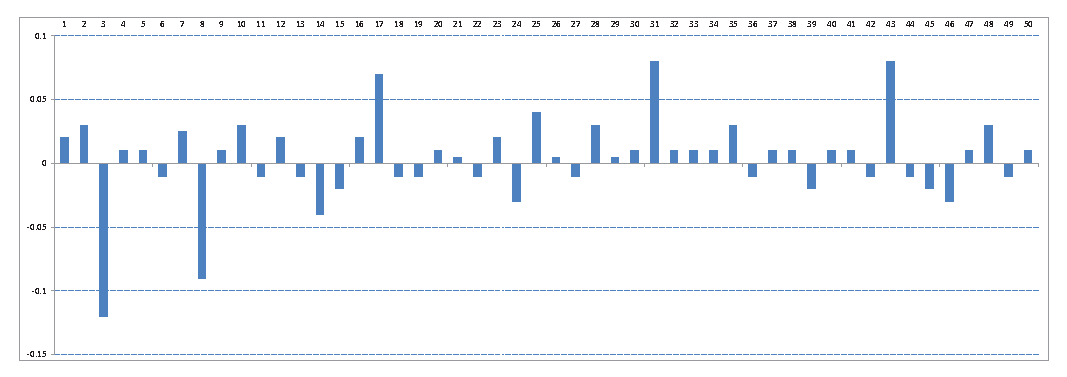
\includegraphics[width=0.9\textwidth]{./figures/topics.eps}
\vspace{-0.7em}
\caption{Topics discussed by two cohorts of users}\label{fig::topic-distribution}}
\vspace{-0.6em}
\end{figure*}








\emph{Topic analysis}. We also extract the underlying topics exists in the corpus and investigate to which extend the content published by AC and NC users are different from each others. We adopted LDA framework as described in Section \ref{sec::topic-content-anal} to extract textual topics from document corpus. Figure \ref{fig::topic-distribution} depicts the differences of the existence of topics across two groups. As you can see from the Figure, the mean change across two groups is $20\%$, which shows two cohorts of users are discussing on different topics online. Specifically, we observe that topics $\#3$ (Self-critical), $\#8$ (Conflicting feelings), $\#17$ (Activities and Sports), $\#31$ (Social support), $\#43$ (Authorized information) show notable variations between two groups. To have a better sense of these topics we listed top $10$ representative words from each topics in Table \ref{table::topics}.  From the Figure \ref{fig::topic-distribution}, following points can be observed. (1) Topic $\#3$ represents `self-critical' contents and the thoughts about being guilty and negative thought about self in NC cohort. This can be attributed into the failure of users in self-managing diabetes and similarly their desire to handle the situation. This is also consistent with the literatures, reporting that chronic disease sufferers develops tendencies of self-criticism which sometimes goes beyond the normal level and may result in mental disorders \cite{anderson2001prevalence,katon1990depression}. (2) Topic $\#8$ represents struggling and conflicting feelings and emotions that are often perceived by NC users. Investigating on the springs and outcomes of this conflicting emotions is worthwhile, which may result to establish better intervention in lifestyle medicine. (3) Discussing about activities and sports is common in AC communities as expressed by topic $\#43$. Indeed a detail checking of extracted topics shows that two other topics which thematically talks about activities ($\#25$, $\#28$); however, they did not show strong distinction between two groups of diabetes. This result verifies the findings from health sciences which states the positive correlation between regular sport activities like `running' and better management of diabetes, especially diabetes Type II\cite{klein2004weight}. It is worth noting that users discussing about sports and exercise activities in social media often utilize tracking devices linked with web portal and mobile applications, which assist them recording the history of their activities and planning for future. The finding is aligned with a recent research reporting that persistent usage of mobile applications significantly increase the success of users in weight loss program~\cite{park2015persistent}. Despite the increasing popularity of tracker devices and mobile applications, limited studies have investigated their impacts and roles in managing chronic diseases, especially diabetes.
(4) Topic $\#31$ describes contents related to social support in online communities. Indeed, \#Bgnow acts as a support groups, or a fast-response, support group for patient with diabetes, where they seek and provide informational and emotional support for their peers. This was already verified by the difference between n-grams usage within two groups. (5) Topic $\#17$ reflects authorized information about diabetes, medications and management programs, showing that diabetic patients in AC groups spread more authorized information about diabetes. In essence, professional health providers leverage the power of social media to disseminate health content for health seekers and AC users republish this information in their network. This highlights another aspects of social media in healthcare.

\begin{table}
\small
\centering
\vspace{-0.2em}
\caption{Examples of topics and corresponding representative words\label{table::topics}}{
\begin{tabular}{|m{0.45cm}|m{4.4cm}|m{2.25cm}|}\hline
\tabincell{c}{ID}&\tabincell{c}{Representative Words}&\tabincell{c}{Topic}\\\hline
\tabincell{c}{T$3$}&\tabincell{c}{tired, hate, missed, hurt, horrible,\\ struggled, sick, damn, ugh, lol}&\tabincell{c}{Self-critical}\\\hline
\tabincell{c}{T$8$}&\tabincell{c}{afraid, want, useless, comfortable,\\ bad, pain, except, tough,\\ nothing, easy}&\tabincell{c}{Conflicting feeling \\ and emotions}\\\hline
\tabincell{c}{T$17$}&\tabincell{c}{running, gym, daily, hypo, mile, \\ ride, walking, sugar,\\ cyclometer, check }&\tabincell{c}{Activities \\ and Sports}\\\hline
\tabincell{c}{T$31$}&\tabincell{c}{talk, dsma, advice, bed, insulin,\\ diet, nutrition, sugar, ask, help }&\tabincell{c}{Social support}\\\hline
\tabincell{c}{T$43$}&\tabincell{c}{research, interested, diet,\\ DiabeticDiary, prove, fact, fitness,\\ food, sleep, hyperglycemia }&\tabincell{c}{Authorized \\ information}\\\hline
\end{tabular}}
\vspace{-0.2em}
\end{table}



\subsection{Visual Content Analysis}
\begin{figure}
 \centering
 \subfigure[]{ \label{fig::AC-samples}
   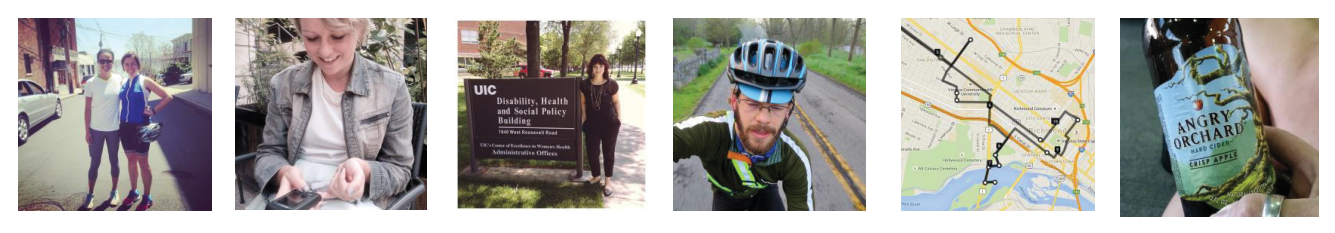
\includegraphics[width=0.48\textwidth]{./figures/AC-samples.eps}}
     \hspace{-1em}
 \subfigure[]{ \label{fig::NC-samples}
   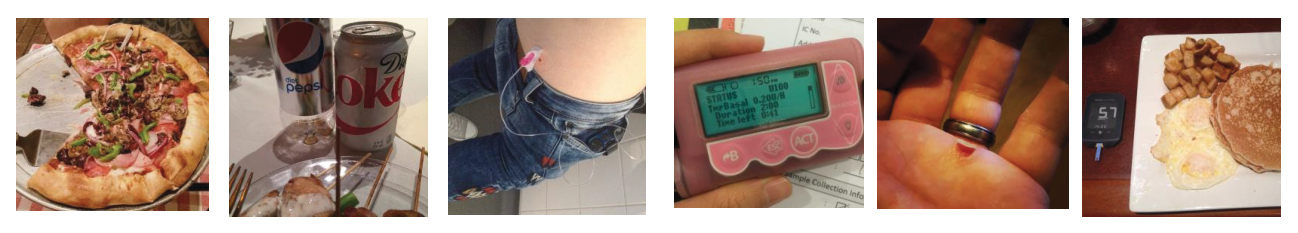
\includegraphics[width=0.48\textwidth]{./figures/NC-samples.eps}}
   \vspace{-0.9em}
   \caption{Exemplar images have been shared by AC users (\textbf{a}), and NC users (\textbf{b}).}
\label{fig::visual-samples} %% label for entire figure
 \vspace{-1em}
\end{figure}

Figure \ref{fig::visual-samples} shows some representative images from the images which have been shared by two groups of users. Our analysis demonstrates that the visual consents in shared images of users' Instagram accounts are highly related to the success of users in managing his diabetes. Figure \ref{visual-concepts} depicts top $20$ statistically significant correlations between visual concepts and the category of users. Several interesting signals can be observed from the Figure. For example, the visual concepts `mountain bike' and `unicycle' are positively correlated to AC category which demonstrates the strong preference of AC users to manage their diabetes with lifestyle change. Some other concepts like `sunglasses', `crash helmet', and `street sign' which are objects related to activities are also demonstrate the same preferences. Retrospective research have also reported similar results in obesity and fitness related studies from social media platforms~\cite{}. Conversely, visual concepts `menu', and `plate` are correlated to NC users, which illustrates the possible reason for failing to control their blood glucose level. Further, the positive correlation between the visual concept `Band Aid' and NC users may indicate that they like to share the picture of their injection site, e.g. insulin injection or pump site, which shows their anxiety related to their health condition.



\begin{figure}
\centering
{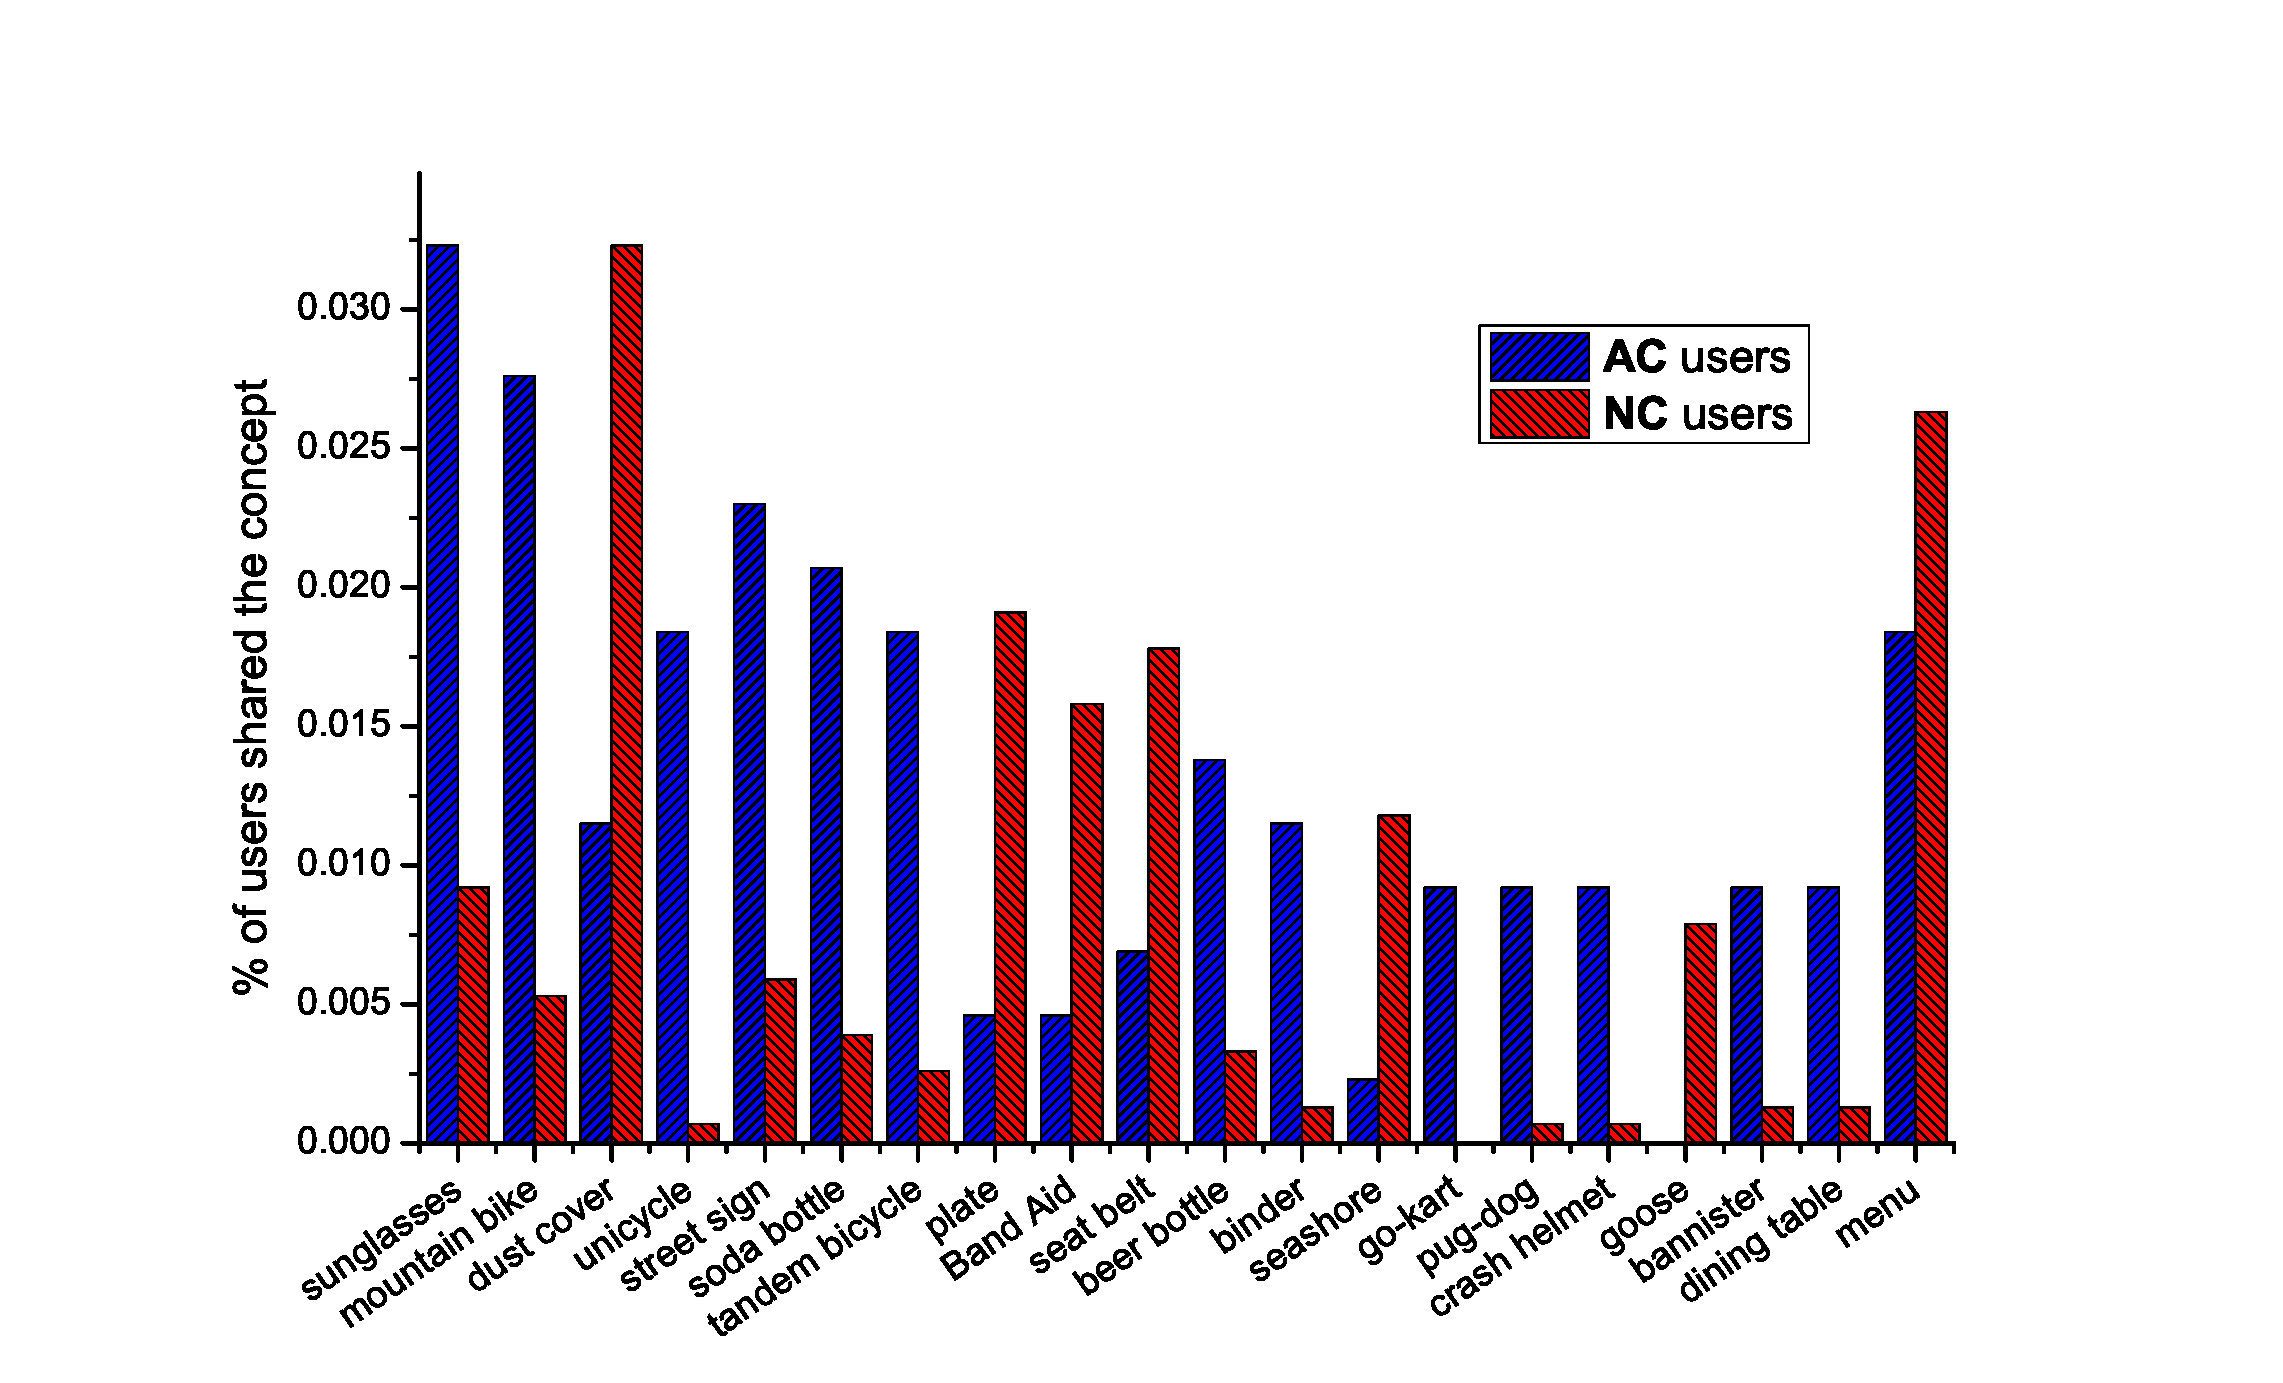
\includegraphics[width=0.51\textwidth]{./figures/visual-concepts.eps}
\vspace{-0.7em}
\caption{Visual concepts which commonly shared by two cohorts of users: AC, and NC users.}\label{visual-concepts}}
\vspace{-0.6em}
\end{figure}

\section{Success Prediction of Diabetes Management}
Success prediction is the task of predicting whether a specific user can successfully maintain his/her health indicators in a suggested range. In this paper, we aim to predict the success of a diabetic patient in controlling his blood glucose value, i.e., he/she belongs to the AC or NC group. In wellness domain, success prediction is an important task and many downstream decisions, such as interventions, treatments, and medications,  are strongly related to the success of the patient in the current procedure/treatment. Here, we considered the success prediction as a binary classification problem in which we predict the category of users between AC and NC groups.

% The prediction task is beneficial in the following scenarios. First, detecting the stage of the user permits us to provide him personalized services based his difficulties and experiences. For example, by connecting non-adopted users to adopted ones, we can assist them to control their diabetes through sharing experiences with their peers. Second, analyzing the discriminant features and machine learning model provides us better understanding and insights on differences in behaviours between AC and NC users. In this section, we first formally defined our problem and then we detail the machine learning approach for predicting the success of users.

To accomplish this end, we use different behavioural attributes studied in last sections as individual features for training and evaluation in a supervised learning method. Each patient is represented with a vector of features and classified into one of two groups. We utilize a linear Support Vector Machine (SVM) as a binary classifier with default setting of scikit-learn \footnote{http://scikit-learn.org/}. For all experiments, we reported the average performance of $10$ random experiments  based on $10$-fold cross validation. Table \ref{table::prediction-performance} demonstrates the performance of different approaches in terms of precision, recall, and F$1$ metrics. To better understand the performance of each attribute, we reported the performance of each behavioral attributes individually and the aggregation of all features. As can be seen from the table, `N-grams' outperformed the two other features `LIWC' and `Latent Topics'. This may be attributed to the fact that n-grams can better capture the semantic context of the text messages. `Latent Topics' demonstrates the lowest performance which is expected since high level semantic topics fail to capture all aspects of text messages.

\begin{table}
\small
\centering
\vspace{-0.2em}
\caption{The performance of different features settings for success prediction task\label{table::prediction-performance}}{
\begin{tabular}{|c|c|c|c|}\hline
\tabincell{c}{}&\tabincell{c}{Precision}&\tabincell{c}{Recall}&\tabincell{c}{F$1$} \\\hline
\tabincell{c}{LIWC}&\tabincell{c}{$59.57$}&\tabincell{c}{$62.46$}&\tabincell{c}{$60.18$} \\\hline
\tabincell{c}{N-grams}&\tabincell{c}{$60.15$}&\tabincell{c}{$63.00$}&\tabincell{c}{$60.41$} \\\hline
\tabincell{c}{Topics}&\tabincell{c}{$53.41$}&\tabincell{c}{$55.14$}&\tabincell{c}{$52.01$} \\\hline
%\tabincell{c}{Visuals}&\tabincell{c}{Acc}&\tabincell{c}{Prec}&\tabincell{c}{Rec}&\tabincell{c}{F$1$} \\\hline
\tabincell{c}{All}&\tabincell{c}{$75.22$}&\tabincell{c}{$71.36$}&\tabincell{c}{$71.21$} \\\hline
\end{tabular}}
\vspace{-0.2em}
\end{table}

%\begin{table}
%\small
%\centering
%\vspace{-0.2em}
%\caption{The performance of different features settings for success prediction task\label{table::prediction-performance}}{
%\begin{tabular}{|c|c|c|c|c|}\hline
%\tabincell{c}{}&\tabincell{c}{Precision}&\tabincell{c}{Recall}&\tabincell{c}{Accuracy}&\tabincell{c}{F$1$} \\\hline
%\tabincell{c}{LIWC}&\tabincell{c}{$59.57$}&\tabincell{c}{$62.46$}&\tabincell{c}{$58.54$}&\tabincell{c}{$60.18$} \\\hline
%\tabincell{c}{N-grams}&\tabincell{c}{$60.15$}&\tabincell{c}{$63.00$}&\tabincell{c}{$61.50$}&\tabincell{c}{$60.41$} \\\hline
%\tabincell{c}{Topics}&\tabincell{c}{$53.41$}&\tabincell{c}{$55.14$}&\tabincell{c}{$54.31$}&\tabincell{c}{$52.01$} \\\hline
%%\tabincell{c}{Visuals}&\tabincell{c}{Acc}&\tabincell{c}{Prec}&\tabincell{c}{Rec}&\tabincell{c}{F$1$} \\\hline
%\tabincell{c}{All}&\tabincell{c}{$75.22$}&\tabincell{c}{$71.36$}&\tabincell{c}{$73.24$}&\tabincell{c}{$71.21$} \\\hline
%\end{tabular}}
%\vspace{-0.2em}
%\end{table}


\section{Discussion}
Our findings reveal several characteristics of social media, specifically Twitter, for diabetes. Many of our finding aligns with prior studies, stating that social media is a rich platform for health consumers through which they seek and share health information. Overall, they demonstrate that people online behaviour expose their health conditions and states as well as their success in adopting their life style to their wellness condition. Waving together these observation, it demonstrates that patient generated wellness data on social media can be effectively utilized for designing better intervention programs and services to assist patienta in better management of their diabetes.
%\subsection{Caveats}
%\subsection{Implications}
\subsection{Clinical Relevance}
The abundant amount of available data can also assist us to better understand patient behaviours and detect potential issues resulting failures in self-management of diabetes. From a clinical perspective, social media can be utilized to complement patient self-report diaries by implicitly tracking his/her online behaviour. Social media can also assist to provide intervention through non-intrusive assessment of content providing and publishing, as discussed below.

\textbf{Persuasion Oriented Intervention}.
With a proper lifestyle and behavioural change, we can successfully manage several chronic diseases such as diabetes, and obesity. While it seems an easy task, in practice, changing lifestyle is a challenging and complex task. According the Fogg Behavioural Model (FBM), three elements need to converge together in order to a behaviour occur: motivation, ability, and trigger~\cite{fogg2010behavior}. Indeed, when a behaviour does not occur, one of these element is missing. Chronic disease sufferers usually have enough motivation to perform the target behaviour, which is suggested by the management program; however, they frequently will not trigger to perform the task on the correct time, e.g. reduce their sugar consumption or their sedentary lifestyle. By utilizing social networks not only we can understand the user lifestyle and wellness condition, but, more importantly, it is possible to motivate the user and trigger him in the same time. For example, we can suggest him some interesting outdoor activity based on his past preferences or suggest him to have a more healthier meal. Further, providing useful health information regarding his/her health condition can effectively motivate user to follow the disease management program, in our case of the diabetes management program.

\textbf{Social Influence Intervention}. In psychology, social influence theory attests that individual's emotions, opinions, and behaviours are affected by others. Social influence has been studied in different domains and environments such as sales, marketing, leadership, and so on \cite{kelman1958compliance}. The holistic concept of wellness traditionally has been studied from different aspects includes, physical, mental, social, and spiritual components.  Late studies extends these perspective to the social interactions finding that social interactions may affect individual's wellness either in positive and negative manner. For example, recent studies have revealed that person's circle of friends may influence his/her weight\cite{shoham2012actor} and his/her sport activity level, i.e., how active he/she is in sports. Upon these findings, we can assist NC diabetics users to better manage their health condition through connecting them to AC users, i.e. diabetic users who already find how to successfully manage their disease.

\subsection{Ethics and Limitations}
While thinking about designing intervention programs on social network and in general health, it is important to bear in mind that wellness and health data can be extremely sensitive and need to be verified before providing to the user. Finding the authorized and reliable wellness information is a challenging task especially in a noisy platform such as social media with a lot of user generated contents and spams contents. The truthworthy of the information needs to be consider with a proper automatic or semi-automatic way. This can be done by a human in loop procedure to verify the potential risky unreliable information. Further, the design consideration in social platforms should honor the privacy of the affected individuals and abide the proper ethical guidelines ensuring that the intended profit of the intervention exceeds the potential difficulties and risks. To sum, we hope this research open a new avenue to not only detect and help diabetic patients through social platforms, but also understand the collaborative behaviour of different diabetics communities towards designing better healthcare interventions and treatments.

It is worthwhile noting that our paper does not make any claim to attributing the social network as an individual platform through which we can obtain a complete understanding of wellness condition of diabetic users and provide a full intervention program. We however attest that patient generated wellness and lifestyle data on social media can be utilized as a complementary source through which we can sense users wellness and lifestyle. Social sensors can be utilized as a complementary source of information in combination of the popular concept of quantified-self measuring users' attributes with wearable devices. We caution against using this method as standalone technique for diagnosis and prediction of diabetes. We also note that social media is a noisy and sparse platform where many users may not utilize it for health information explicitly; however, the implicit signals and clues in their social account can provide useful information when aggregated in scale.

Finally, our findings reveals the richness of patient generated wellness data on social media demonstrating that it can be used in combination of other information sources to obtain a comprehensive understanding of diabetes patient. It also raise several difficult questions for researchers, as mentioned below. How much social media information are reliable in health domain? How precise user's online behaviour reveal his offline attributes and behaviours? and How effective would the designed intervention be, in terms of changing user behaviour?
%\subsection{Caveats}

\section{Conclusions and Future Work}
%Social media is continually used as a platform for sharing, seeking, and discussing around health challenges, transforming these platforms as a source for knowledge, support, and engagement for patient living with chronic diseases. Studying behavioural characteristic and the language of users online can offer invaluable insights on how health consumers interacts and influence each other on social networks. In this paper, we investigate to characterize the differences between language and behaviour of diabetic users on Twitter microblogging platform. In particular, we aim to investigate the behavioural distinction between patients who can successfully manage their diabetes and those who fail. We study patient behavioural online in terms of linguistic, textual and visual attributes and contents in their online posts. We observed several characteristics such as negative affective, seeking and sharing supportive contents, and difference in shared visual concepts, which differs adopted and non-adopted users. We discuss the implication of our finding in providing better healthcare intervention and provide a supervised model which can predict the success of user based on his published online content.

Social media is continually used as a platform for informational and emotional support around health challenges transforming these platform as a source for knowledge, support and engagement for patients living with chronic diseases such as diabetes. In such a context patients are encouraged to shared the exact values of their health measurements such as blood glucose level. In this paper, we aim to study the behavioural distinction of two groups of diabetes patient based on their published posts online. In particular, we investigate the behavioural distinction between patients who can successfully manage their blood glucose value and those who fail. We observed several distinction in terms of linguistic, textual and visual contents of published posts online. We also provide a supervised approach to predict the success of users based on his online behaviour.
	

\bibliographystyle{abbrv}
\footnotesize
\bibliography{Diabetes}
\end{document}
